\documentclass[12pt,a4paper]{article}
\usepackage[swedish,english]{babel}
\usepackage[T1]{fontenc}
\usepackage[utf8]{inputenc}
\usepackage{graphicx}
\usepackage{mathtools}
\usepackage{subcaption}

\graphicspath{ {images/} }

\author{
  Matstoms, Axel
  \and
  Jankovi\'{c}, Luka
  \and
  Matstoms, Ivar
}

%\date{2018-03-15}

\title{GAMLP: En symbolhanterare}

\begin{document}
\selectlanguage{swedish}
\maketitle
\begin{figure}[h]
  \centering
  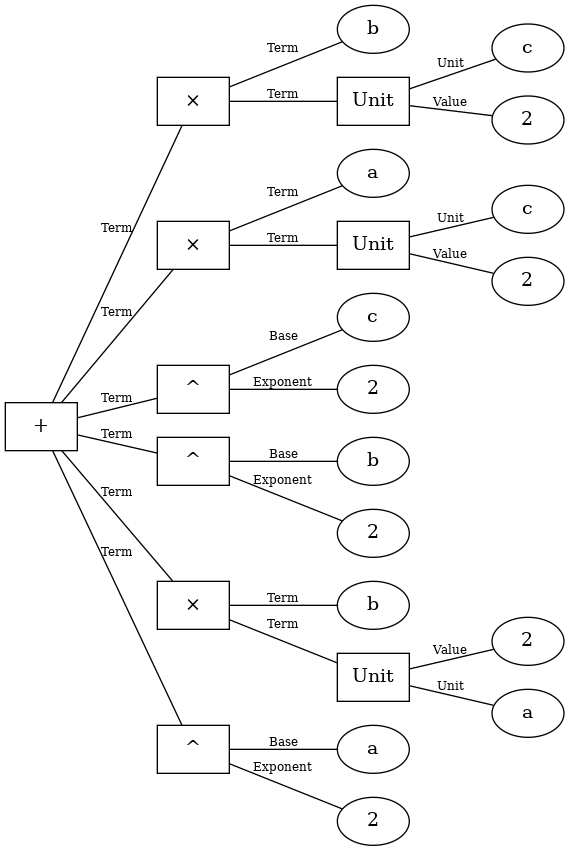
\includegraphics[width=0.7\textwidth]{image27}
  %\caption{Välj en olämplig bild}
\end{figure}
\newpage
\selectlanguage{english}
\begin{abstract}
The purpose of this project is to look at some of the techniques used by sites such as WolframAlpha to simplify algebraic expressions and solve particular kinds of equations. To research this we wrote an application in Python with some of the features of such sites.  We chose to work with Python because of how quickly code can be written in Python and due to the fact everybody in the group knew Python before the project even started. During the span of this project we were able to develop an application which is able to take input and construct an abstract syntax tree which is then simplified. The application is able to handle many of our goals set in the beginning, including addition and multiplication of polynomials correctly, although not always fully simplified. The application is also able to solve polynomials up to the second degree. With time the application could easily be expanded to cover more aspects of what we set out to do such as polynomial division and solving polynomial equations of higher grades.ga
\end{abstract}
\textbf{Keywords:} Abstract syntax tree; Python; Algebraic Expressions
\selectlanguage{swedish}
\newpage
\tableofcontents
\newpage
\section{Inledning}
Eftersom vi alla i gruppen delar en stor passion för programmering ville vi göra något som kombinerar programmering med ett naturvetenskapligt ämne. Vi övervägde flera olika projekt, bland annat en realtids fysikmotor, implementationer av matematiska funktioner (såsom sinus, exponenter) på hårdvarunära nivå samt idén som valdes: en symbolhanterare. En symbolhanterare, eller CAS, Computer Algebra System, är ett datorprogram som kan mata in, tolka, och lösa ekvationer, exempelvis \(5x + 10 = 20\). En annan funktion som en symbolhanterare antar är förmågan att förenkla uttryck, exempelvis \((x + 2)(x - 3) \Leftrightarrow (x^{2} - x - 6)\). Skillnaden mellan en vanlig miniräknare och en symbolhanterare är att symbolhanterare förstår algebra och kan samt kan hantera variabler, inte bara värden.
\section{Teori}
\subsection{Abstrakt syntaxträd}
Det är besvärligt för ett program att tolka ekvationer som är skrivna på vanlig form (e.x. \(5x + 10 = 15\)). Därför är det viktigt att ekvationen först byggs upp på ett sätt som är mer hanterbart för ett datorprogram. Så kallade abstrakta syntaxträd används oftast inom datavetenskap för att strukturera programmeringskod så att en kompilator kan omvandla källkoden till ett exekverbart program. Men på grund av likheterna mellan programmeringsspråkens syntax och matematiska ekvationer användes abstrakta syntaxträd i detta arbete.
\subsubsection{Allmänt om träd}
Inom datavetenskap beskrivs träd som en form av datastruktur för att representera hierarkisk data. Ett träd inom matematiken består av noder som är sammansatta på så vis att varje nod kan innefatta ett eller flera barn, som i sig också är noder. I det här dokumentet kallas barnen för barnnoder eller subnoder. Noder behöver dock ej innefatta några barn, och då kallas dessa noder för löv. Dock behöver varje nod anta ett värde. Detta kan vara t.ex. ett numeriskt värde (e.x. \(5\) eller \(10\)), eller en operation (e.x. addition, multiplikation). Om en nod ej är ett barn till en annan nod betyder det att denna nod är högst upp i trädet. Denna typ av nod kallas för rotnod eller bara rot.
\subsubsection{Implementation av syntaxträd}
Trädet i sig utgår från en rotnod (eng. rootnode). I vårt fall är denna nod alltid ett likhetstecken (\(=\)), eftersom det är där ekvationen utgår ifrån. Precis som t.ex. en operatörsnod kan rotnoden anta två subnoder (I detta fall måste två noder antas, en för VL och en för HL). Därefter kan leden byggas upp av olika sorters noder.
\subsubsection{Noder}
\label{subsubsec:noder}
En nod måste anta ett värde. Detta kan uppnås genom att ge noden ett konkret värde (e.x. \(5\) eller \(10\)), en konstant (e.x. \(\pi\), \(e\)), funktion (e.x. \(log\), \(sin\)) eller operator (e.x. \(+\), \(-\), \(\times\), \(\div\), \string^). Om noden är sådan att den kräver argument, dvs. kräver ett eller flera värden för att själv få ett värde (\(+\) har ej ett värde utan två siffror på vardera sida av sig.) så kan noden själv anta noder (s.k. barnnoder, eng. childnodes) för att uppfylla sitt värde. Se Figur \ref{fig:2131}.
\begin{figure}[h]
  %24
  \centering
  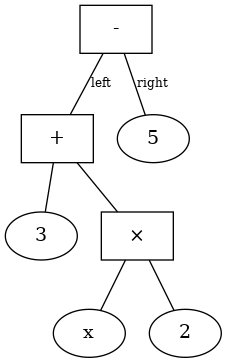
\includegraphics[width=0.3\textwidth]{image24}
  \caption{Visuell representation av \((2x + 3) - 5\) som ett abstrakt syntaxträd.}
  \label{fig:2131}
\end{figure}
Eftersom programmet ska kunna hantera ekvationslösning, måste den okända variabeln kunna representeras (e.x. \(5x + 10 = 20\). Här är \(x\) den okända variabeln). För att representera variabeln används en speciell typ av nod; så kallad enhetsnod. Denna nod antar ett värde (för koefficienten) och en representation av den okända variabeln; en så kallad enhet. Denna enhet består av själva variabeln och vilken grad som den representeras i. Se Figur \ref{fig:2132} för en visuell representation av \(2x^{2}\) som en enhetsnod.
\begin{figure}[h]
  %25
  \centering
  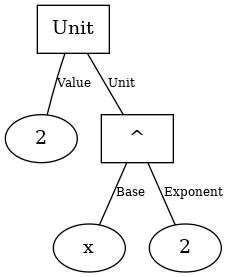
\includegraphics[width=0.3\textwidth]{image25}
  \caption{\(2x^{2}\) representerat som en enhetsnod med enheten \(x^{2}\) och värdet \(2\).}
  \label{fig:2132}
\end{figure}
\subsection{Allmänt om förenkling}
Operatörsnoder vars subnoder endast består av numeriska värden räknas helt enkelt ihop med den operatorn som noden representerar. Då kommer denna operatörsnod ersättas med en nummernod som antar det ihopräknade värdet.
\subsection{Homogena noder}
Homogena noder är de noder där ordningen av subnoder ej spelar någon roll vilket gör att de kan lagras som en lista (array) och är inte limiterad i antal. Dock byggs homogena noder först upp av flera noder med bara två subnoder (Se 2.4 Inhomogena noder) eftersom det är så programmet tolkar inmatningen, se Figur \ref{fig:2311}.
\subsubsection{Allmän förenkling av homogena noder}
\begin{figure}[h]
  %22
  \centering
  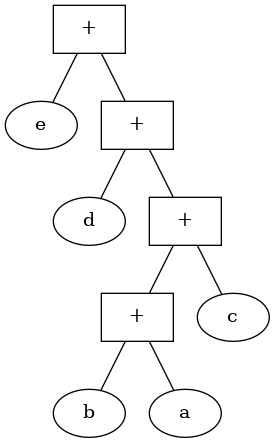
\includegraphics[width=0.3\textwidth]{image22}
  \caption{\((a + b + c + d + e)\) tolkat av programmet.}
  \label{fig:2311}
\end{figure}
Att förenkla noder som precis har tolkats av programmet (se Figur \ref{fig:2311}) är dock opraktiskt. Därför är det första steget i förenklingen att försumma staplade homogena noder av samma typ till en enda nod. Om noderna antar numeriska värden räknas de ihop till en subnod, medans variabler (\(x\)) helt enkelt lämnas som en subnod. Efter det läggs elementen in i noden en efter en och varje element kontrolleras om den kan slås ihop med en annan subnod. Detta gäller dock endast för noder med numeriska värden. Hur enhetsnoder (se \ref{subsubsec:noder} för förklaring av enhetsnod) hanteras är dock olika för varje typ av homogen nod. Därför förklaras detta i detalj i samband med varje typ av nod.\par
Två enhetsnoder med samma enhet kan slås ihop genom att addera värderna.
\begin{figure}[h]
  %16
  \centering
  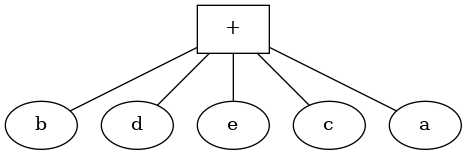
\includegraphics[width=0.5\textwidth]{image16}
  \caption{(a, b, c, d, e) efter första steget av förenkling av homogen nod}
  \label{fig:2312}
\end{figure}
\begin{figure}[h]
%  \begin{subfigure}[h]
%    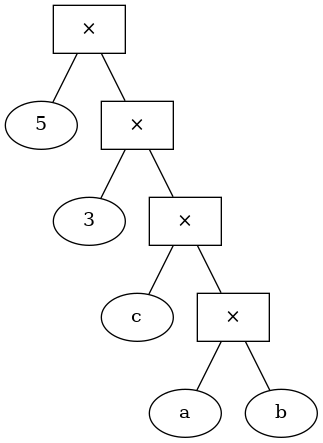
\includegraphics[width=0.3\textwidth]{image23}
%  \end{subfigure}
%  \begin{subfigure}[h]
%    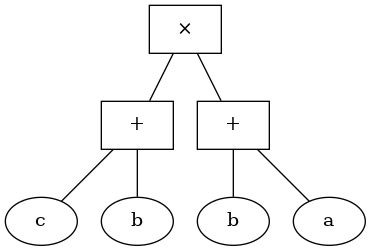
\includegraphics[width=0.3\textwidth]{image26}
%  \end{subfigure}
%  \begin{subfigure}[h]
%    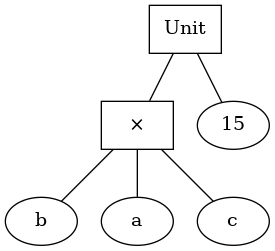
\includegraphics[width=0.3\textwidth]{image19}
%  \end{subfigure}
  \centering
  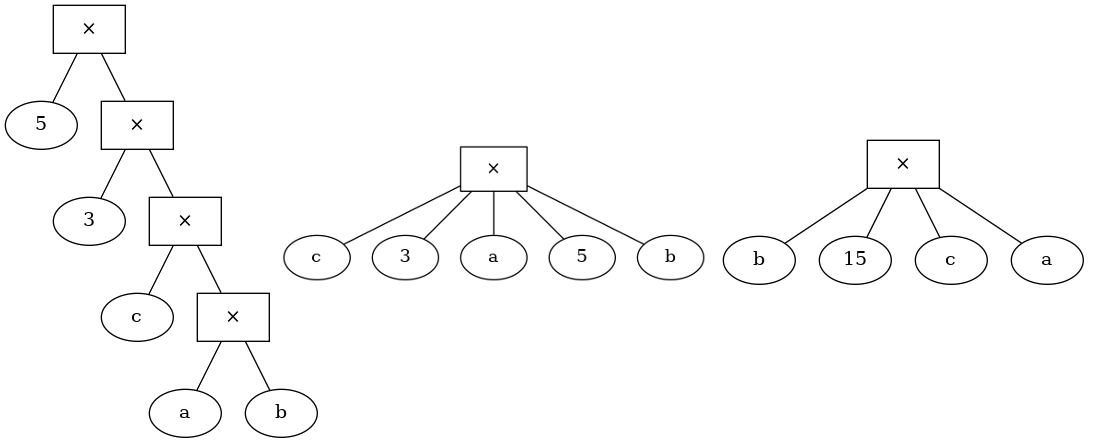
\includegraphics[width=0.9\textwidth]{image-merged}
  \caption{\((a \times b \times c \times 3 \times 5) förenklas i tre steg, a,b,c lyfts upp till samma nod och talen separeras till sin egen nod, tillslut räknas talen ihop.}
  \label{fig:2313}
\end{figure}
\end{document}
